\documentclass{article}
\usepackage{amsmath}
\usepackage{tikz}
\begin{document}
\section*{More precise determination of the bounding boxes of
\texttt{tikzpicture}s}

\subsection*{Current status}

Ti\emph{k}Z determines the bounding box of (cubic) Bezier curves by establishing the
smallest rectangle that contains the end point and the two control points of the
curve (cf.\ Figure~\ref{fig:BoundingBoxBezier}).
\begin{figure}[!htb]
\centering
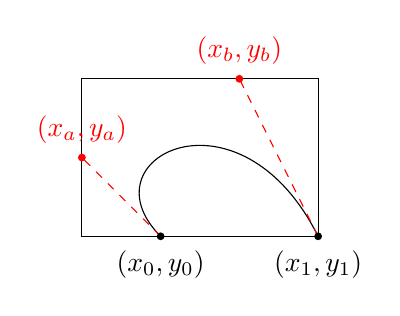
\begin{tikzpicture}[bullet/.style={circle,fill,inner sep=1pt}]
 \draw (0,0)  .. controls (-1,1) and (1,2) .. (2,0);
 \draw (current bounding box.south west) rectangle 
  (current bounding box.north east);
 \draw[red,dashed] (0,0) -- (-1,1) node[bullet,label=above:{$(x_a,y_a)$}]{}
  (2,0) -- (1,2) node[bullet,label=above:{$(x_b,y_b)$}]{};
 \path (0,0) node[bullet,label=below:{$(x_0,y_0)$}]{}
 (2,0) node[bullet,label=below:{$(x_1,y_1)$}]{};
\end{tikzpicture}\quad%
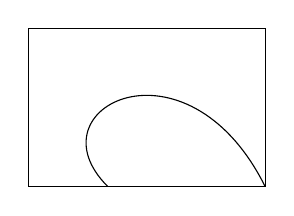
\begin{tikzpicture}
 \draw (0,0) .. controls (-1,1) and (1,2) .. (2,0);
 \draw (current bounding box.south west) rectangle 
  (current bounding box.north east);
\end{tikzpicture}
\caption{Ti\emph{k}Z bounding boxes and an example.}
\label{fig:BoundingBoxBezier}
\end{figure}

This may lead to drastic overestimates of the bounding box (cf.\
Figure~\ref{fig:BoundingBoxExample}).

\begin{figure}[!htb]
\centering
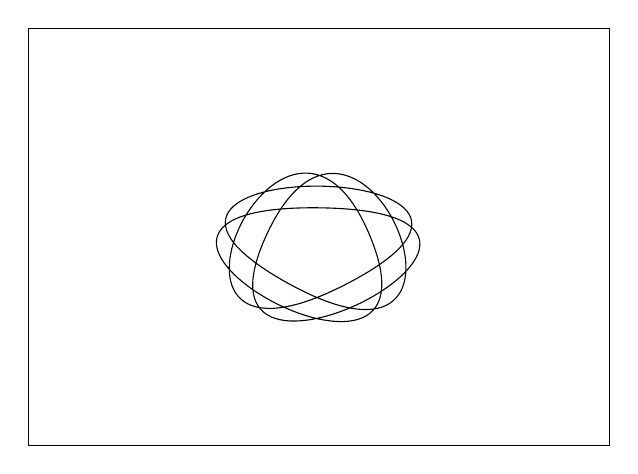
\begin{tikzpicture}[y=0.30pt, x=0.4pt,yscale=-1]
 \path[draw=black,fill=white]
   (258.9527,290.5199) .. controls (173.9885,538.4766) and (568.5860,261.2969) ..
   (306.5098,257.1141) .. controls (44.4337,252.9312) and (429.9845,542.5624) ..
   (352.9767,292.0206) .. controls (275.9689,41.4788) and (119.6549,497.6604) ..
   (334.1376,346.9999) .. controls (548.6203,196.3394) and (66.4622,188.6439) ..
   (276.0276,346.0724) .. controls (485.5930,503.5010) and (343.9169,42.5633) ..
   (258.9527,290.5199) -- cycle;
  \draw (current bounding box.south west) rectangle 
  (current bounding box.north east);
 \end{tikzpicture}
\caption{Example from \texttt{https://tex.stackexchange.com/q/43621/121799}.}
\label{fig:BoundingBoxExample}
\end{figure} 

\clearpage
\subsection*{Computing the bounding box}

Establishing the precise bounding box has been discussed in various places, the
following discussion uses in part the results from
\texttt{https://pomax.github.io/bezierinfo/}. What is a cubic Bezier curve? A
cubic Bezier curve running from $(x_0,y_0)$ to $(x_1,y_1)$ with control points
$(x_a,y_a)$ and $(x_a,y_a)$ can be parametrized by
\begin{equation}
 \gamma(t)~=~
 \begin{pmatrix} x(t)\\ y(t) \end{pmatrix}~=~
 \begin{pmatrix}t^3 x_{1}+3 t^2 (1-t) x_{b}+(1-t)^3
   x_{0}+3 t (1-t)^2 x_{a}\\
   t^3 y_{1}+3
   t^2 (1-t) y_{b}+(1-t)^3 y_{0}+3 t (1-t)^2
   y_{a}\end{pmatrix}\;,\label{eq:gammaBezier}
\end{equation}
where $t$ runs from 0 to 1 (and $\gamma(0)=(x_0,y_0)$ and
$\gamma(1)=(x_1,y_1)$). Surely, the bounding box has to contain
$(x_0,y_0)$ and $(x_1,y_1)$. If the functions $x(t)$ and $y(t)$ have extrema in
the interval $[0,1]$, then the bounding box will in general be larger than that.
In order to determine the extrema of the curve, all
we need to find the extrema of the functions $x(t)$ and $y(t)$ for $0\le t\le
1$. That is, we need to find the solutions of the quadratic equations
\begin{equation}
 \frac{\mathrm{d}x}{\mathrm{d}t}(t)~=~0\quad\text{and}\quad
 \frac{\mathrm{d}y}{\mathrm{d}t}(t)~=~0\;.
\end{equation}
Let's discuss $x$, $y$ is analogous. If the discriminant
\begin{equation}
 d~:=~x_{0} x_{1}-x_{0}
   x_{b}-x_{1}
   x_{a}+x_{a}^2-x_{a}
   x_{b}+x_{b}^2
\end{equation}
is greater than 0, there are two solutions
\begin{equation}
 t_\pm~=~\frac{x_{0}-2
   x_{a}+x_{b}\pm\sqrt{x_{0} x_{1}-x_{0}
   x_{b}-x_{1}
   x_{a}+x_{a}^2-x_{a}
   x_{b}+x_{b}^2}}{x_{0}-x_{1}-3
   x_{a}+3 x_{b}} \;.
\end{equation}   
In this case, we need to make sure that the bounding box contains, say
$(x(t_-),y_0)$ and $(x(t_+),y_0)$. If $d\le0$, the bounding box does not need to
be increased in the $x$ direction. One can plug $t_\pm$ back into
\eqref{eq:gammaBezier}, this yields
\begin{subequations}
\begin{align}
x_-&~=~\frac{x_0^2x_1 + x_0x_1^2 - 3x_0x_1x_a + 6x_1x_a^2 + 
  2x_a^3 - 3(x_0 + x_a)(x_1 + x_a)x_b + 
  3(2x_0 - x_a)x_b^2 + 2x_b^3 - 
  2\Delta(x_0x_1 - x_1x_a + x_a^2 - (x_0 + x_a)x_b + 
    x_b^2)}{(x_0 - x_1 - 3x_a + 3x_b)^2}\;,\\
x_+&~=~\frac{x_0^2x_1 + x_0x_1^2 - 3x_0x_1x_a + 6x_1x_a^2 + 
  2x_a^3 - 3(x_0 + x_a)(x_1 + x_a)x_b + 
  3(2x_0 - x_a)x_b^2 + 2x_b^3 + 
  2\Delta(x_0x_1 - x_1x_a + x_a^2 - (x_0 + x_a)x_b + 
    x_b^2)}{(x_0 - x_1 - 3x_a + 3x_b)^2}\;,
\end{align}
\end{subequations}
where
\begin{align}
\Delta&~=~\sqrt{x_0x_1 - x_1x_a + x_a^2 - (x_0 + x_a)x_b + x_b^2}\;.
\end{align}



As already mentioned, the analogous
statements apply to $y(t)$. 

It is rather straightforward to implement this
prodecure in Ti\emph{k}Z. The relevant macros are \verb|\pgf@lt@curveto| (and
\verb|\pgf@nlt@curveto|).\footnote{Some care has to be taken when squaring
lengths since they are all measured in points, and the square can easily become
large and trigger a \texttt{dimension too large} error. When computing the
discriminant $d$, I thus divided these distances by some taming factor that I
took to be 32 for no special reasons. It might very well be that there are
better taming factors, or that one needs to dial the taming factor as a function
of the input values.} The macro \verb|\pgf@lt@curveto| takes six arguments,
which are $x_a$, $y_a$, $x_b$, $y_b$, $x_1$ and $y_1$ (in that order). $x_0$ and
$y_0$ are stored in \verb|\pgf@path@lastx| and \verb|\pgf@path@lastx|,
respectively.

\subsection*{Examples}

\makeatletter
\def\pgf@lt@curveto#1#2#3#4#5#6{%
  % extrema in x
  \pgfmathparse{((#1/32)*(#1/32)-1*((#1/32)*(#3/32))+(#3/32)*(#3/32)-1*((#1/32)*(#5/32))+(-(#3/32)+(#5/32))*(\pgf@path@lastx/32))}%
  \pgfutil@tempdima=\pgfmathresult pt % <- why do I need this space?
  \ifdim\pgfutil@tempdima>0pt%
   \pgfmathsetmacro{\tone}{min(1,max(0,(\pgf@path@lastx-2*#1+#3-32*sqrt(\pgfutil@tempdima))/(\pgf@path@lastx-#5-3*#1+3*#3)))}%
   \pgfmathparse{\pgf@path@lastx*pow(1-\tone,3)+3*#1*pow(1-\tone,2)*\tone+3*#3*(1-\tone)*\tone*\tone+#5*pow(\tone,3)}%
   \pgf@protocolsizes{\pgfmathresult pt}{#6}%
   \pgfmathsetmacro{\tone}{min(1,max(0,(\pgf@path@lastx-2*#1+#3+32*sqrt(\pgfutil@tempdima))/(\pgf@path@lastx-#5-3*#1+3*#3)))}%
   \pgfmathparse{\pgf@path@lastx*pow(1-\tone,3)+3*#1*pow(1-\tone,2)*\tone+3*#3*(1-\tone)*\tone*\tone+#5*pow(\tone,3)}%
   \pgf@protocolsizes{\pgfmathresult pt}{#6}%
  \fi% 
  % extrema in y
  \pgfmathparse{((#2/32)*(#2/32)-1*((#2/32)*(#4/32))+(#4/32)*(#4/32)-1*((#2/32)*(#6/32))+(-(#4/32)+(#6/32))*(\pgf@path@lasty/32))}%
  \pgfutil@tempdima=\pgfmathresult pt % <- why do I need this space?
  \ifdim\pgfutil@tempdima>0pt%
   \pgfmathsetmacro{\tone}{min(1,max(0,(\pgf@path@lasty-2*#2+#4-32*sqrt(\pgfutil@tempdima))/(\pgf@path@lasty-#6-3*#2+3*#4)))}%
   \pgfmathparse{\pgf@path@lasty*pow(1-\tone,3)+3*#2*pow(1-\tone,2)*\tone+3*#4*(1-\tone)*\tone*\tone+#6*pow(\tone,3)}%
   \pgf@protocolsizes{#5}{\pgfmathresult pt}%
   \pgfmathsetmacro{\tone}{min(1,max(0,(\pgf@path@lasty-2*#2+#4+32*sqrt(\pgfutil@tempdima))/(\pgf@path@lasty-#6-3*#2+3*#4)))}%
   \pgfmathparse{\pgf@path@lasty*pow(1-\tone,3)+3*#2*pow(1-\tone,2)*\tone+3*#4*(1-\tone)*\tone*\tone+#6*pow(\tone,3)}%
   \pgf@protocolsizes{#5}{\pgfmathresult pt}%
  \fi% 
  \pgf@protocolsizes{\the\pgf@path@lastx}{\the\pgf@path@lasty}%
  \pgf@protocolsizes{#5}{#6}%
  \pgfsyssoftpath@curveto{\the#1}{\the#2}{\the#3}{\the#4}{\the#5}{\the#6}%
}
\let\pgf@nlt@curveto\pgf@lt@curveto
\makeatother 

\begin{figure}[!htb]
\centering
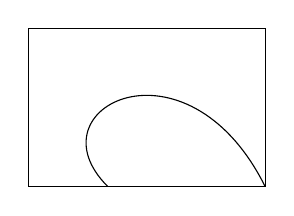
\begin{tikzpicture}
 \draw (0,0) .. controls (-1,1) and (1,2) .. (2,0);
 \draw (current bounding box.south west) rectangle 
  (current bounding box.north east);
\end{tikzpicture}
\caption{Tight bounding box for figure~\ref{fig:BoundingBoxBezier}.}
\end{figure}

\begin{figure}[!htb]
\centering
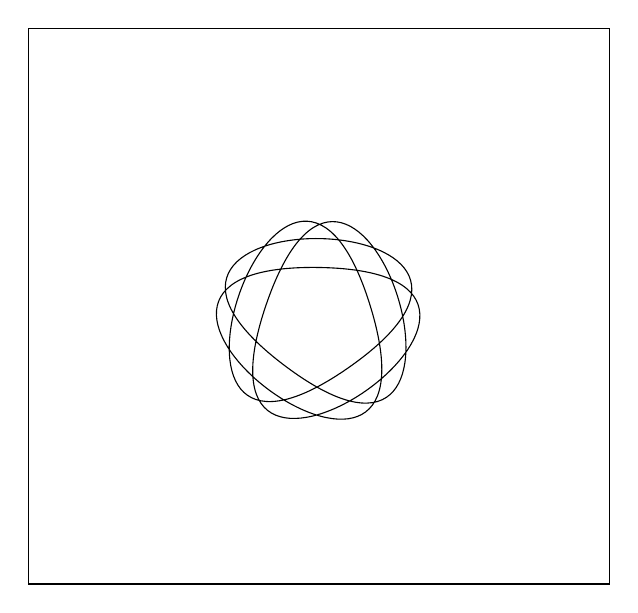
\begin{tikzpicture}[y=0.40pt, x=0.4pt,yscale=-1]
 \path[draw=black,fill=white]
   (258.9527,290.5199) .. controls (173.9885,538.4766) and (568.5860,261.2969) ..
   (306.5098,257.1141) .. controls (44.4337,252.9312) and (429.9845,542.5624) ..
   (352.9767,292.0206) .. controls (275.9689,41.4788) and (119.6549,497.6604) ..
   (334.1376,346.9999) .. controls (548.6203,196.3394) and (66.4622,188.6439) ..
   (276.0276,346.0724) .. controls (485.5930,503.5010) and (343.9169,42.5633) ..
   (258.9527,290.5199) -- cycle;
  \draw (current bounding box.south west) rectangle 
  (current bounding box.north east);
\end{tikzpicture}
\caption{Tight bounding box for figure~\ref{fig:BoundingBoxExample}.}
\end{figure}
\end{document}
